%!TEX root = ../main/main.tex

La siguiente tabla resume las probabilidades de absorción $P_{abs}$ y transmisión $P_{trans}$ del problema para distintos números de historias simuladas $N_{hist}$. 

\begin{table}[h!]
	\centering
	\begin{tabular}{|c|c|c|}
		\hline
		$N_{hist}$ & $P_{abs}$        & $P_{trans}$      \\ \hline
		1.000           & $0.98900 \pm 0.00959$ & $0.01100 \pm 0.00233$ \\ \hline
		100.000         & $0.99161 \pm 0.00109$ & $0.00839 \pm 0.00027$ \\ \hline
		10.000.000      & $0.99185 \pm 0.00011$ & $0.00815 \pm 0.00003$ \\ \hline
	\end{tabular}
	\caption{Resultados del modelo}
\end{table}

Se recuerda que las restricciones del problema están dadas por enunciado, las cuales son las siguientes:


\begin{table}[h!]
	\centering
	\begin{tabular}{|c|c|c|c|}
		\hline
		Región & $\Sigma_t$ & $\Sigma_a$ & Espesor      \\ \hline
		Núcleo & $0.05$ & $0.005$ & $0.5$ \\ \hline
		Cascarón 1 & $0.1$ & $0.01$ & $0.1$ \\ \hline
		Cascarón 2 & $10.0$ & $0.1$ & $0.1$ \\ \hline
		Cascarón 3 & $100.0$ & $10.0$ & $0.1$ \\ \hline
	\end{tabular}
	\caption{Restricciones del problema}
\end{table}

\begin{figure}[h!]
	\centering
	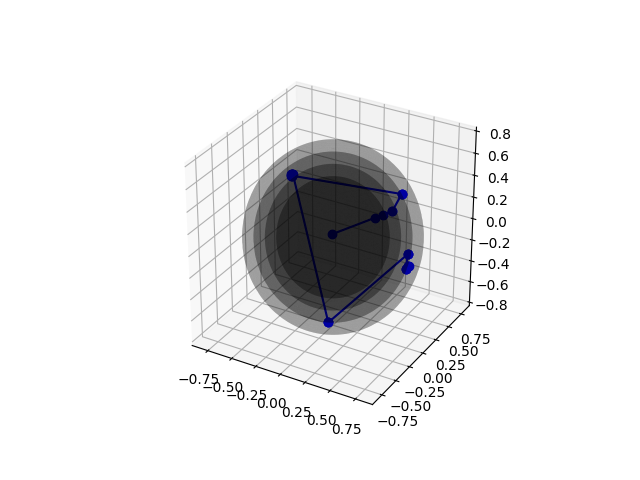
\includegraphics[width=0.7\linewidth]{fig1}
	\caption{Ejemplo de historia graficada en la geometría del problema}
\end{figure}


Podemos notar que la probabilidad de absorción es muy grande para los constreñimientos dados, lo que se condice con lo esperado, dado que en las capas exteriores el camino libre medio recorrido por la partícula entre cada interacción es muy pequeño, por lo que es muy probable que ocurran muchas interacciones antes de que la partícula escape de la geometría. La probabilidad de absorción, dado que ocurre una interacción, es siempre del $10\%$ para cada región, entonces lo que limita la transmisión de las partículas es la sección eficaz $\Sigma_t$.\\

Utilizando el \emph{script} adjunto a esta entrega escrito en lenguaje Python, \texttt{check.py}, es posible verificar esto. El \emph{script} lo que hace es revisar una historia al azar (entregada solo sí el programa principal \texttt{main.c} se ajusta para que entregue un \emph{output}) y graficarla en la geometría del problema. En la figura 2 se puede apreciar un \emph{output} del \emph{script} mencionado, podemos ver que a medida que la partícula se aleja del núcleo (y entra a los cascarones más grandes) el número de interacciones aumenta considerablemente, este comportamiento se encuentra en la gran mayoría de las historias simuladas.\\

Por otro lado, como es de esperarse, mientras mayor es la cantidad de historias simuladas más preciso es el resultado, los errores calculados a base de dispersión estadística de los \emph{batches} de simulación se ajustan de manera consistente a el valor. Se afirma así que, a medida que se aumenta el número de historias, el valor de $P_{abs}$ y $P_{trans}$ convergen cada una a un cierto número, tal y como se esperaría por la Ley de los Grandes Números.